\section{Non-linear system dynamics}\label{sec:chaos}
\subsection{Introduction to chaos}
In the world of classical mechanics the formalism presented by Hamilton offered a means of describing the dynamical behaviour of the world we observe. Not limited to the classical world, Hamiltonian mechanics naturally describes the quantum world also, which forms the basis for quantum mechanics. If restricted to linear systems, the behaviour of a dynamical process using this approach
can often be easily interpreted and analysed. However, given a non-linear system in Hamiltonian mechanics, the behaviour may become much more complex, giving rise to dynamics not observable in linear systems. The study of such non-linear processes is important in many areas of physics. The Gross--Pitaevskii equation is a non-linear form of the Schr\"{o}dinger equation, and can describe much richer physical dynamics than its linear counterpart.

To examine all possible states in a dynamical system, it is often best to consider the use of phase--space methods. For a system described by Hamiltonian mechanics, we consider for a 1D classical particle a set of coordinates consisting of the position, $q$, and the momentum, $p$. Thus, the phase--space for the particle extends over a 2D coordinate space, or 2N-dimensions for N particles. For a variety of differing initial states, the behaviour observed in phase space can consist of closed orbits, such as in the case of a simple harmonic oscillator. However, an important point to note is that in higher dimensions, initially neighbouring orbits can diverge exponentially from one another over time. The rate at which these states diverge can be described by the function $\exp(\lambda t)$, where $\lambda$ is known as the Lyapunov exponent \cite{BK:Kibble_2004}. Given a positive value for $\lambda$, the resulting behaviour of the system is termed to be ``chaotic'', and therefore strongly dependent on the initial conditions.

\subsection{Chaotic systems}\label{ss:chaotic}
An important note about chaotic systems is that the behaviour arises from non-linear effects only. Non-linear systems with a phase-space dimensionality of three or greater can exhibit complex dynamical behaviour which is unobservable in their linear counterparts. Chaotic behaviour tends to allow the trajectories in phase--space to move from closed orbits to seemingly random trajectories. More informally, chaotic behaviour in classical systems is often defined as the inability to predict the outcome of a particular system behaviour \cite{CT:Gardiner_pra_2000}. Although an exact definition differs from author to author, the following statements are often used as a means to classify chaotic behaviour in the context of dynamical systems \cite[p. 323]{BK:Strogatz_1994}
\begin{itemize}
	\item The Lyapunov exponent is positive, resulting in diverging trajectories for infinitesimally small differences in initial conditions. This can be stated as a sensitivity to initial conditions.\vspace*{-0.5em}
	\item The system under examination must be deterministic, with chaotic behaviour arising solely from the non-linearity, not random (noisy) inputs.\vspace*{-0.5em}
	\item The long term behaviour of trajectories should not settle.
\end{itemize}

One of the ways to describe whether a system is chaotic or not comes from the integrability of the system. If there are the same number of
conserved quantities, $M$, as pairs of coordinates, $N$, then the system can be described as integrable. For such an integrable system, all subsequent motion can occur only within an invariant torus of $N$--dimensions. However, without this integrability condition, the motion may occupy $2N-M$ dimensional space, where $M<N$. In this case, the predictability of the system's motion becomes difficult, with the system entering a chaotic regime. Since we are dealing with systems of dimension three and greater, methods for visualising the resulting dynamics in phase--space are difficult. One solution is the use of a Poincar\'e section, which allows the projection of a high-dimensional phase-space onto a 2D/3D plot. Non-integrable systems will fill the area of the resulting Poincar\'e section, whereas integrable systems will show closed orbits. The area-filling property of non-integrable systems is often used as a sign for the presence of chaos in the system.

\begin{figure}[tb]
\centering
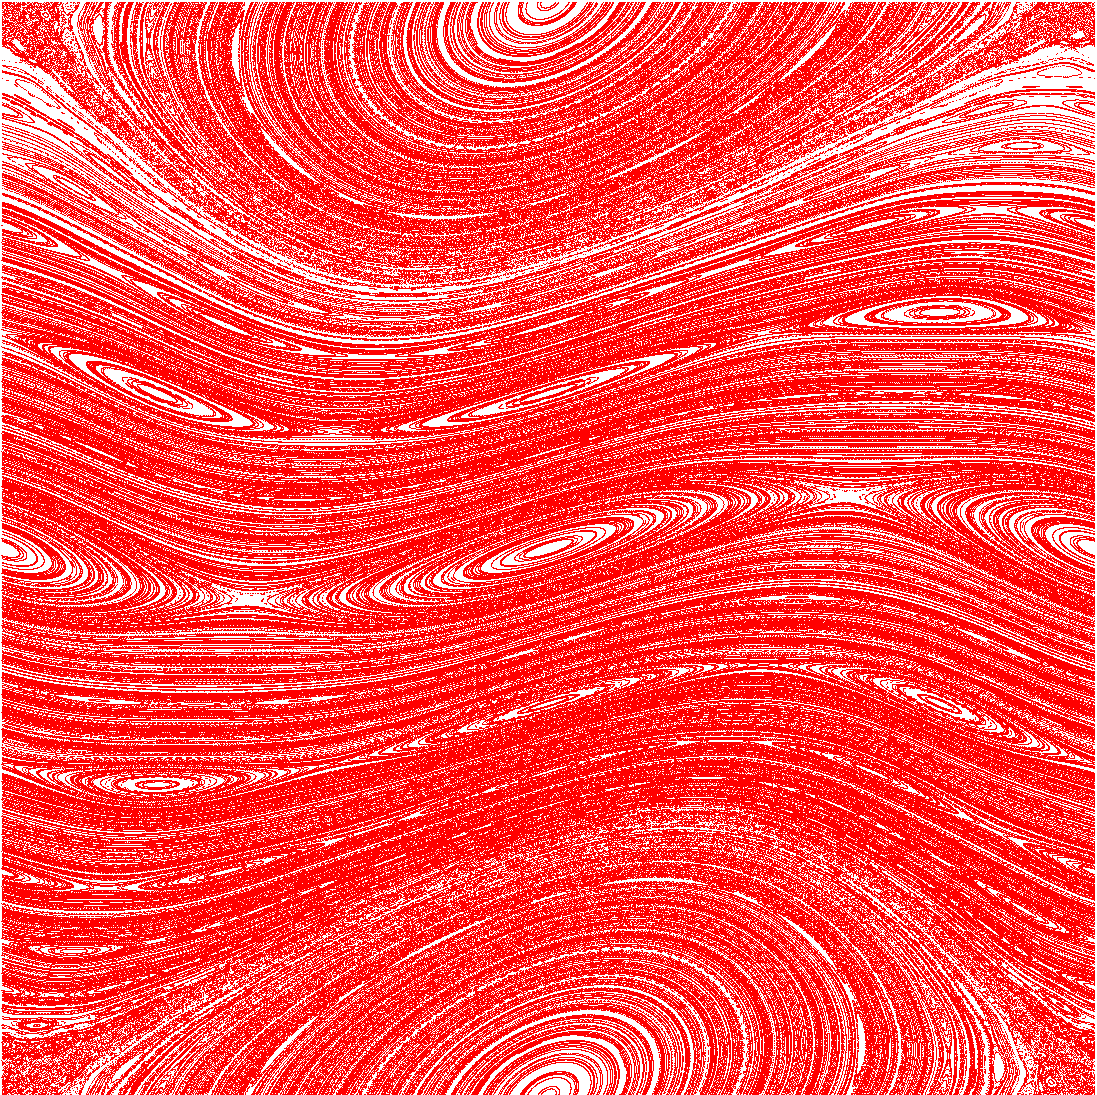
\includegraphics[scale=0.13,trim=0cm 0cm 0cm 0cm]{ch1_litrev/k_0_6.png}
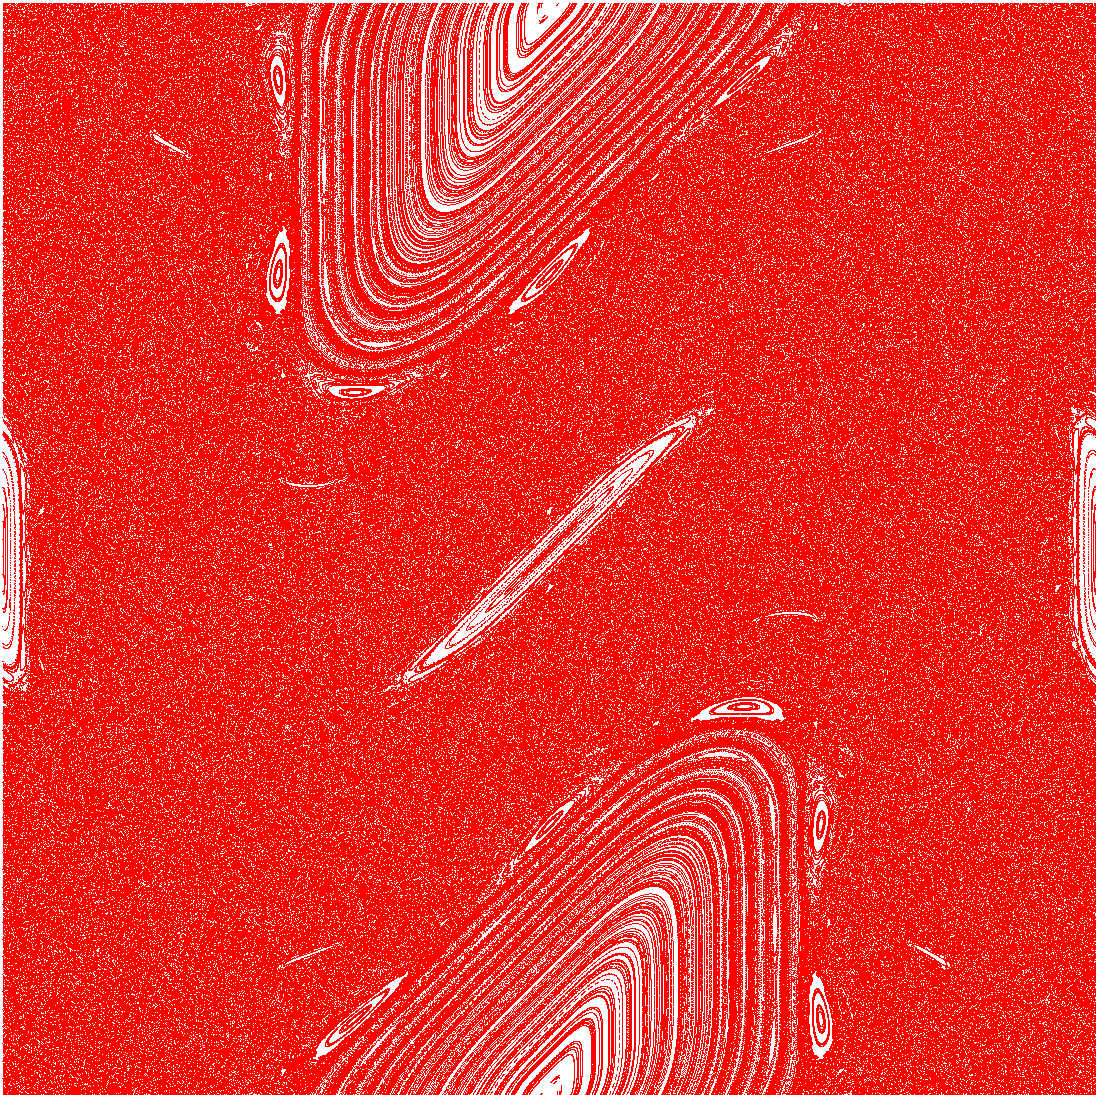
\includegraphics[scale=0.13,trim=0cm 0cm 0cm 0cm]{ch1_litrev/k_2_0.png}
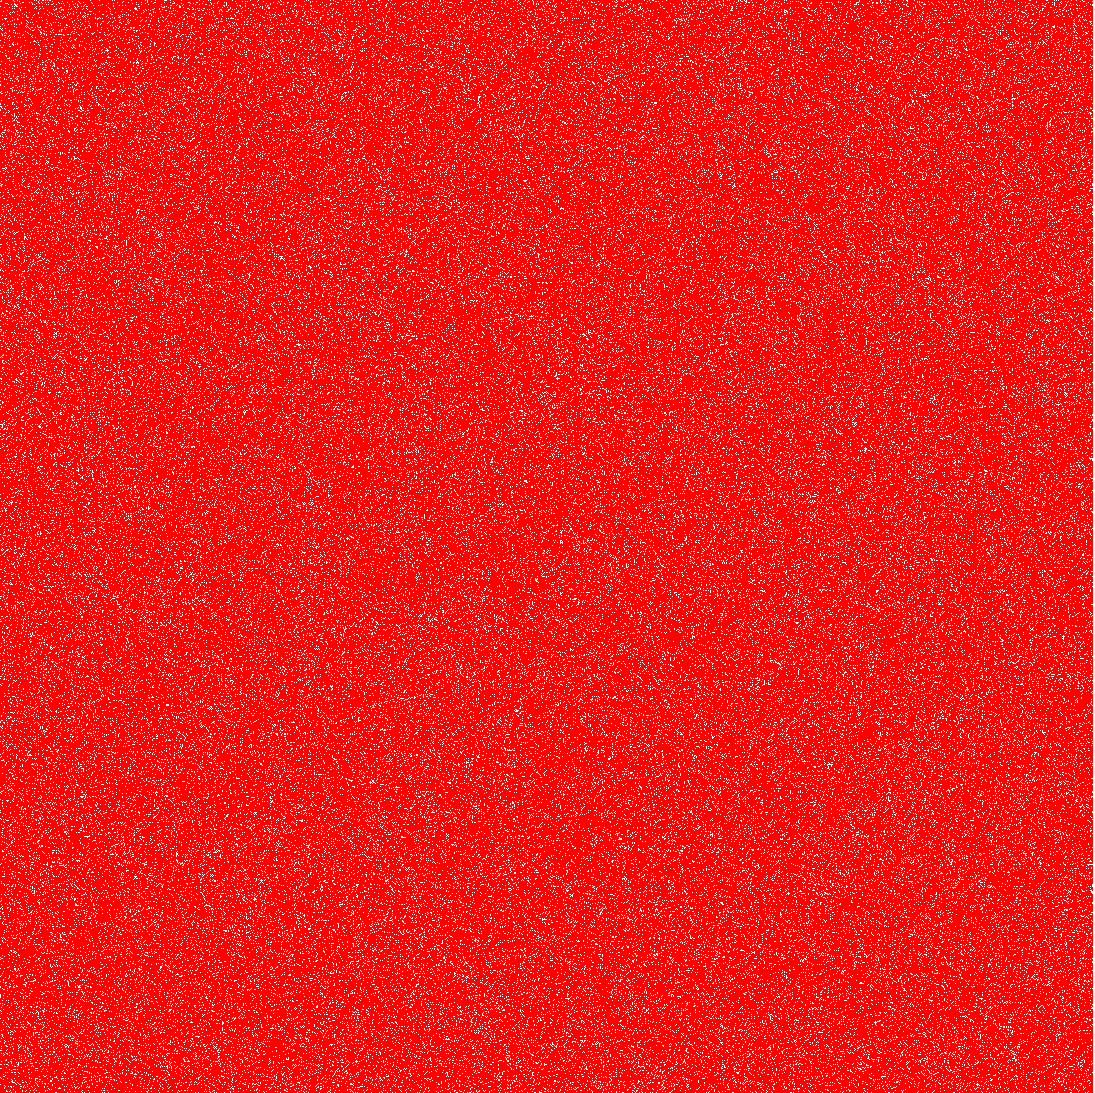
\includegraphics[scale=0.13,trim=0cm 0cm 0cm 0cm]{ch1_litrev/k_12_0.png}
\caption{Images left to right represent phase space states of the classical kicked rotor using the standard map with increasing kicking strength, $K$. The left panel corresponds to $K=0.6$, still showing trajectories; the middle panel is for $K=2.0$, which shows chaos and 3 visible orbit regions; the right panel shows $K=12.0$ yielding a completely chaotic state.}
\label{fig:kickedrotor}
\end{figure}

One widely used model applied to understand such dynamics is that of the kicked rotor \cite{CT:Korsch_ajp_2008}. This model can be thought of as a particle rotating about a fixed point on a ring, receiving periodic kicks, the relative strength and sign of which depend upon the position on the ring. The variables in such a model are the momentum, $p$, which can take any value, and the angle, $\theta$, which is confined to values between 0 and 2$\pi$. The Hamiltonian describing such a system is given by
\begin{equation} \label{eqn:kickedrotor}
H = \frac{p^2}{2m} - K\cos(\theta)\displaystyle\sum_{n=-\infty}^{\infty}\delta(t-n\tau),
\end{equation}
where $K$ represents the kicking strength, and $\delta$ is the Dirac delta function, with $\tau$ being the kicking period. This type of system has been extensively used to understand both classical and quantum chaotic behaviour \cite{CT:Ulah_thesis_2012}. Examples for the trajectories for differing kicking strengths, $K$, are given in Fig. \ref{fig:kickedrotor}. It is easy to see that low kicking strengths give closed orbits, whilst an increase in kicking strength allows the system to enter a globally chaotic regime. The images in the chaotic regime demonstrate the area-filling property of the Poincar\'e section in phase--space.

A related system offering similar behaviour is the delta kicked harmonic oscillator, which modifies the Hamiltonian defined by Eq. \eqref{eqn:kickedrotor}, to include an additional harmonic potential. The resulting Hamiltonian is
\begin{equation}\label{eqn:deltaharmosc}
H = \frac{p^2}{2m} + \frac{m\omega^2 x^2}{2} - K\cos(kx)\displaystyle\sum_{n=-\infty}^{\infty}\delta(t-n\tau),
\end{equation}
where $\omega$ is the frequency of the harmonic potential, and $k=2\pi/\lambda$ is the wavenumber of the periodic potential.  This model can be thought of as a classical particle in a harmonic potential, oscillating and receiving periodic kicks with the strength and sign dependent upon the position within the potential. Gardiner \cite[chap. 4]{THS:Gardiner_2000} discusses this model, and the resulting chaotic behaviour for the classical case and for the quantum case. Variation of the kicking strength and period leads to a variety of interesting dynamics, and the onset of chaos can be observed as the kicking strength increases.

\subsection{Chaos in quantum systems}
The statements characterising chaos given in Section \ref{ss:chaotic} are applicable to classical systems only. One significant difference is that the sensitivity to initial conditions is no longer given due to the unitary nature of the quantum operators \cite{CT:Schack_pre_1996,CT:Gardiner_pra_2000}. The connection between classical chaotic behaviour and quantum mechanics, therefore, remains to be understood as the correspondence principle, given by Bohr, states that quantum dynamics has to reproduce classical dynamics in certain limits. However, classically chaotic systems do not show a quantum counterpart. The hypersensitivity to initial conditions does not appear in quantum systems, and quasiperiodic quantum systems can have a fully chaotic classical equivalent system \cite{CT:Jensen_nat_1992}. As such, the term ``quantum chaos'' has come to refer to
quantum systems which can be described by a Hamiltonian exhibiting chaos in a classical setting. The quantum delta kicked harmonic oscillator, previously described for classical systems, has been studied for its ability to generate chaotic dynamics in works given by Daly \cite{THS:Daly_1994}, Gardiner \cite{THS:Gardiner_2000}, and Kells \textit{et al}. \cite{CT:Kells_pre_2004}. Given the requirement of non-integrability to observe chaotic dynamics, it is worth noting that in the limit where the Schr\"{o}dinger equation is valid the system can be integrable due to its linear nature \cite{THS:Gardiner_2000}. The quantum delta-kicked harmonic oscillator dynamics can be examined by replacing the classical conjugate variables, $(x,p)$, of the Hamiltonian Eq. \eqref{eqn:deltaharmosc}, with their quantum operators, $(\hat{x},\hat{p})$, as
\begin{equation}\label{eqn:hamiltonian_qkick}
\hat{H} = \frac{\hat{p}^2}{2m} + \frac{m\omega^2 \hat{x}^2}{2} - K\cos(k\hat{x})\displaystyle\sum_{n=-\infty}^{\infty}\delta(t-n\tau).
\end{equation}
The dynamics in such a quantum system can be examined using similar tools as the ones presented for classical systems, such as phase-space visualisation. Obtaining a phase-space representation of the wavefunction is, however, not as straightforward as in the classical case. A common method for this involves calculating the Wigner quasiprobability function from the wavefunction.

Experimentally realisable systems that can exhibit such behaviour have recently become accessible, with the delta kicked rotor having been implemented in an optical and condensate system \cite{CT:Ullah_epjd_2012,CT:Lemos_natcomm_2012}. Such systems are, however, still rare. The extension of the above Hamiltonian to non-linear systems described by the Gross--Pitaevskii equation, rather than the linear Schr\"{o}dinger equation, opens up the possibility of observing interesting dynamics. Given that the area of quantum chaos is not as developed as that of classical chaos, the literature is not as well formulated, and tends to be more qualitative than quantitative, barring a few works. The use of Floquet theory is required to fully understand how to analyse periodic quantum chaotic systems, as it is a widely used method applied to describe the quantum behaviour \cite{CT:McCaw_thesis_2005}. Mapping a system onto the Hamiltonian as, for example, the one given by Eq. \eqref{eqn:hamiltonian_qkick}, would provide a way to realise a system that can yield observable chaotic behaviour. For this reason, the proposal given in Section \ref{sec:prelim} will discuss using this Hamiltonian as an integral part of my PhD thesis research.
